\documentclass[10pt,a4paper,sans]{moderncv}

\moderncvstyle{banking}
\moderncvcolor{red}
\nopagenumbers{}

\usepackage[utf8]{inputenc}
\usepackage[scale=0.75]{geometry}
\usepackage{fontawesome}
\usepackage{import}
\usepackage[absolute,overlay]{textpos}

\patchcmd{\makehead}
  {\setlength{\makeheaddetailswidth}{0.8\textwidth}}
  {\setlength{\makeheaddetailswidth}{\textwidth}}
  {}
  {}

% % personal data
\firstname{Marius-Danut} 
\familyname{Iancu}
\title{Curriculum Vitae}                        
%\address{, , , , }{}{}
\phone[mobile]{0728 296 475}                   
\email{marius.danut94@outlook.com}                                
\social[linkedin]{MariusDanutIancu}
\social[github]{MariusDanutIancu}
%\extrainfo{}                          
\quote{}                                 

\begin{document}

	\hskip -3cm {\makecvtitle}
	\begin{textblock}{0}(12.75,1)
		\fboxsep=1mm
		\fboxrule=1pt
		\fcolorbox{red}{white}{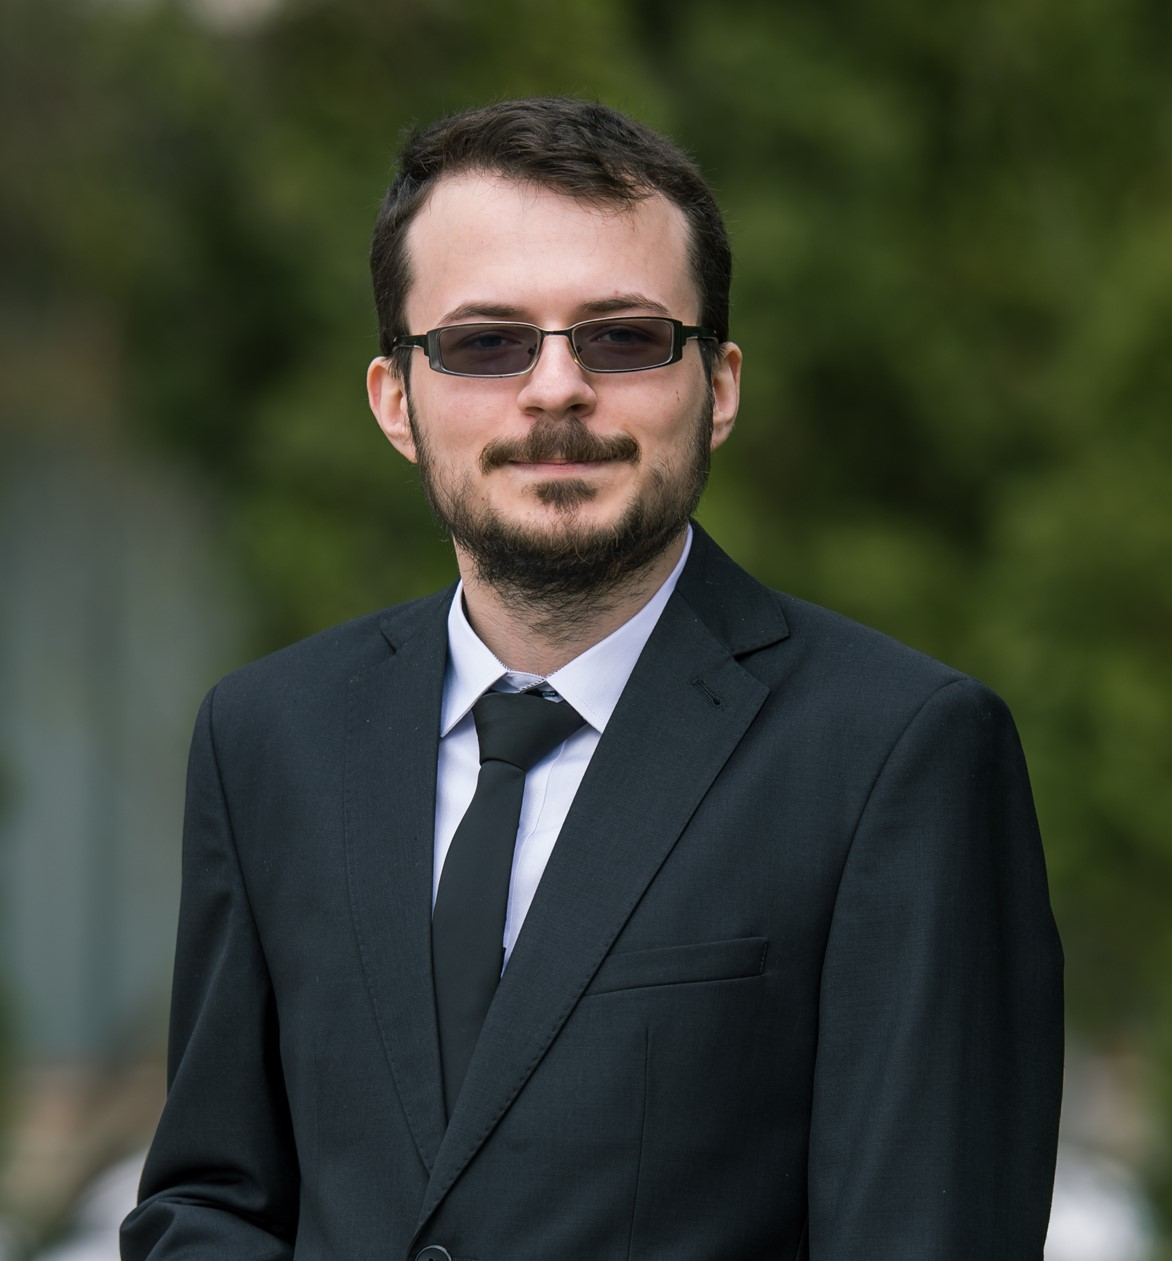
\includegraphics[width=3.5cm]{images/avatar.jpg}}
	\end{textblock}

	%\small{Intro}
	
	\section{Objective}	
		\vspace{5pt}
		\small{To pursue a challenging career and be part of a progressive organization that helps to enhance my knowledge, skills and hence grow and excel along with the organization.} 

	%\section{Previous Employment}
		%\vspace{5pt}
		%\begin{itemize}
			%\item{A}{B}{C}{D}{E}{{F}}
		%\end{itemize}
	
	\section{Education}
		
		\vspace{5pt}
		\subsection{Academic Qualifications}
			
			\begin{itemize}

				\vspace{2pt}
				\item{\cventry{2014--2018}{Faculty of Computer Science}{University: "Alexandru Ioan Cuza" din Iasi}{Iasi}{\textit{-}}{}}
				\vspace{2pt}
				\item{\cventry{2009--2013}{Maths/Computer science - intensive}{National College: "Mihail Sadoveanu"}{Pascani}{\textit{-}}{}}

			\end{itemize}
		
		\vspace{5pt}
		\subsection{Notable Projects}
			
			\begin{itemize}
				\vspace{2pt}
				\item{\textbf{Bachelor's thesis  (2018) \textit{"Lung cancer detection using Neural Networks"} }\textit{(Supervisor: Madalina Raschip) }}
				\small{}
			\end{itemize}

			\begin{itemize}
				\vspace{2pt}
				\item{\textbf{Fii Practic (2018) \textit{"SpringBoot Healthcare REST Application"} }\textit{(Supervisor: tss-yonder)}}
				\small{}
			\end{itemize}
			
	\section{Technical and Personal skills}
		\begin{itemize}

			\vspace{5pt}
			\item \textbf{Programming Skills:}  Python, C++, C, Java, Android, SQL, HTML, CSS
			
			\vspace{2pt}
			\item \textbf{Operating Systems:} Windows, Ubuntu
			
			\vspace{2pt}
			\item \textbf{Applications:} Microsoft Visual Studio, Microsoft Office, Android Studio, Intellij idea, PyCharm, Unreal Engine, Maya
			
			\vspace{2pt}
			\item \textbf{Database systems:} Sqlite, Mysql, Oracle
			
			\vspace{2pt}
			\item \textbf{Frameworks:} Spring Boot (Java), Flask (Python)

			\vspace{2pt}
			\item \textbf{Version control:} Git
			
			\vspace{2pt}
			\item \textbf{Languages:} Romanian, English
			
		\end{itemize}
	
	\section{Interests and extra-curricular activity}
		\begin{itemize}
			\vspace{5pt}
			\item \textbf{Interests}: Artificial Intelligence, Deep learning, Healthcare, Emerging technologies
			\vspace{2pt}
			\item \textbf{Extra-curricular activity}: Listening music, Travelling, Surfing the Internet, Asian culture
		\end{itemize}
	
	\section{Relevant Courses:}
		\begin{itemize}
			\vspace{5pt}
			\item \textbf{Faculty of Computer Science: }Object oriented programming, Advanced programming, Python programming, Databases, Computer Networks, 
			Artificial Intelligence, Operating systems, Information security, Numerical Calculus, Machine Learning, Artificial neural networks
			\vspace{5pt}
			\item \textbf{Datacamp: }Python programming and data science courses
		\end{itemize}
	
	% \section{References}
	\clearpage
\end{document}
